\section{Results}

This section presents the evaluation results organized into four main parts:
Section~\ref{sec:environment} details the testing environment and hardware
specifications; Section~\ref{sec:presentations-results} presents scalability
results for the \texttt{Presentations} data model;
Section~\ref{sec:stocks-results} analyzes performance with the more complex
\texttt{Stocks} data model; and Section~\ref{sec:memory-analysis} provides
detailed memory consumption and resource utilization analysis.

\subsection{Environment Specifications}
\label{sec:environment}

All benchmarks were conducted on a GitHub-hosted virtual machine under GitHub
Actions, running Ubuntu 24.04.2 LTS with an AMD EPYC 7763 64-Core Processor
(x86\_64 architecture) operating at 3.24 GHz, configured with 2 CPU cores and 2
threads per core, and 7.8 GB of available RAM. The system utilizes a 75 GB SSD
with ext4 filesystem, achieving 1.5 GB/s write throughput in basic I/O tests.
Network connectivity is provided through a 1500 MTU Ethernet interface. All
tests were conducted on OpenJDK 21 (Corretto build) with the G1 garbage
collector enabled by default. The JVM arguments used were: \texttt{-Xms512m
     -Xmx16g}. Each test was executed 5 times per configuration to ensure result
reliability.

All template engines were configured to use UTF-8 encoding and disable
automatic HTML escaping to ensure fair comparison and consistent output across
all template engines. Caching behaviour was left as the default for each
engine, allowing them to optimize template loading and rendering as per their
design. These configurations ensure that all engines operate under equivalent
conditions, with template loading, encoding, and escaping behavior normalized
across implementations.

For both the Apache Bench and JMeter tests, we simulate a 1000-request warmup
period for each route with a concurrent user load of 32 users. The warmup
period is followed by the actual test period, during which we simulate 256
requests per user, scaling in increments up to 128 concurrent users.

The results are presented in the form of throughput (number of requests per
second) for each template engine, with the x-axis representing the number of
concurrent users and the y-axis representing the throughput in requests per
second.

Both Quarkus and Spring MVC implementations were configured with an 8KB output
buffer size to ensure consistency, despite Quarkus not enabling PSSR at this
size and Spring MVC not supporting PSSR for the tested templates. Testing with
a reduced 512B buffer size showed only a 0.046\% performance difference with
Rocker, indicating negligible impact. Both frameworks use unlimited platform
thread pools, enabling on-demand thread creation up to system limits for
maximum throughput and scalability observation under high concurrent load.

Since the obtained results for JMeter and Apache Bench show no significant
differences, only the JMeter results will be presented. Statistical analysis of
test configurations revealed an average absolute percentage difference of
2.83\% between the two load testing tools. While individual approach
differences ranged from -16.53\% to +14.66\% at the extremes, the consistent
directional bias and small magnitude of differences indicate that both tools
provide comparable performance measurements. Given this statistical equivalence
and the need for brevity, only JMeter results are presented, as they provide
representative performance characteristics across all tested configurations.

\subsection{Scalability results for the \texttt{Presentations} class} \label{sec:presentations-results}

The results in Figure~\ref{fig:presentations-webflux-jmeter} depict the
throughput (number of requests per second) for each template engine, with
concurrent users ranging from 1 to 128, from left to right. The benchmarks
include HtmlFlow using suspendable web templates (\textit{HtmlFlow-Susp},
equivalent to the approach shown in Listing~\ref{lst:presentation-flow}),
Jstachio using Virtual Threads with the \texttt{Iterable} interface
(\textit{Jstachio-Virtual}), and Thymeleaf using the reactive View Resolver
driver (Thymeleaf-Rx). \textit{Blocking} and \textit{Virtual} represent the
average throughput of the blocking approaches (i.e., KotlinX, Rocker, Jstachio,
Pebble, Freemarker, Trimou, HtmlFlow, and Thymeleaf) when run in the context of
a separate coroutine dispatcher or Virtual Threads, respectively.

We show the \textit{HtmlFlow-Susp}, \textit{Jstachio-Virtual}, and
\textit{Thymeleaf-Rx} engines separately to observe the performance of the
non-blocking engines when using the Suspending, Virtual Thread, and Reactive
approaches. The \textit{Blocking} and \textit{Virtual} are aggregated due to
the similar performance of different engines when using those approaches.

\begin{figure}[h]
     \centering
     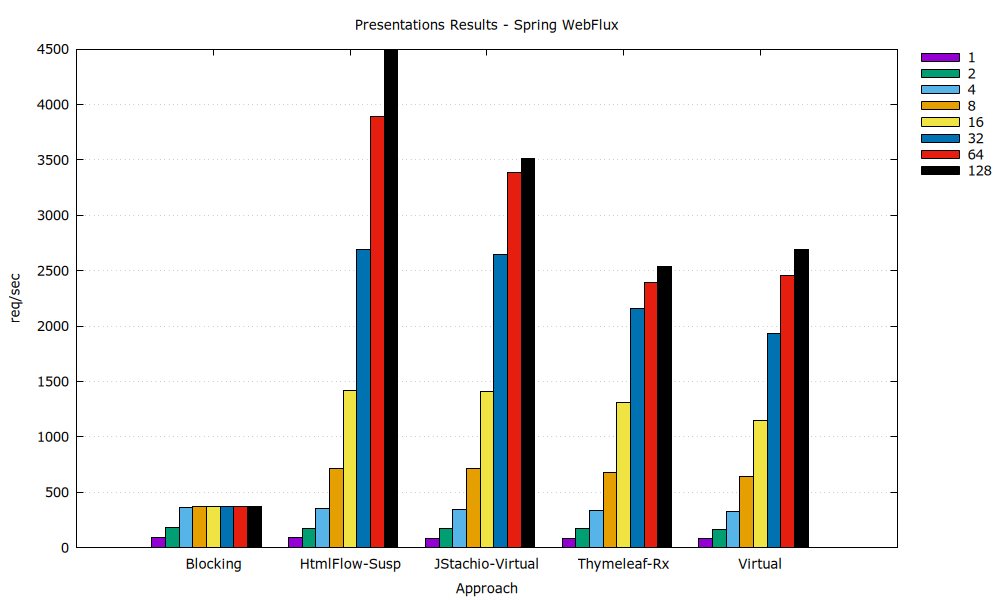
\includegraphics[width=0.8\textwidth]{./Graphs/presentations-webflux-jmeter.png}
     \caption{Throughput (requests per second) scalability results for Spring Webflux with \texttt{Presentations} class}\label{fig:presentations-webflux-jmeter}
\end{figure}

The results in Figure~\ref{fig:presentations-webflux-jmeter} show that when
using blocking template engines with a separate coroutine dispatcher, the
engines are unable to scale effectively beyond 4 concurrent users. In contrast,
\textit{HtmlFlow-Susp} scales up to 128 concurrent users, achieving 4,487
requests per second. When blocking approaches are executed in the context of
Virtual Threads—thus enabling non-blocking I/O—the engines scale up to 64
concurrent users, with Jstachio using Virtual Threads reaching 3,514 requests
per second. The Thymeleaf implementation using the reactive View Resolver
driver scales up to 32 concurrent users, achieving a lower maximum throughput
of 2,559 requests per second.

It is important to note that the differences in scalability and throughput
between the \textit{HtmlFlow-Susp}, \textit{Jstachio-Virtual}, and
\textit{Thymeleaf-Rx} approaches may be influenced by the specific template
engines used, rather than the approach itself. When comparing the
\textit{Reactive}, \textit{Suspendable}, and \textit{Virtual} approaches
specifically with HtmlFlow, we found that all three achieve similar
performance: HtmlFlow using a blocking approach with Virtual Threads reaches
4,691 requests per second, while HtmlFlow using a reactive approach achieves
4,792 requests per second.

\begin{figure}[h]
     \centering
     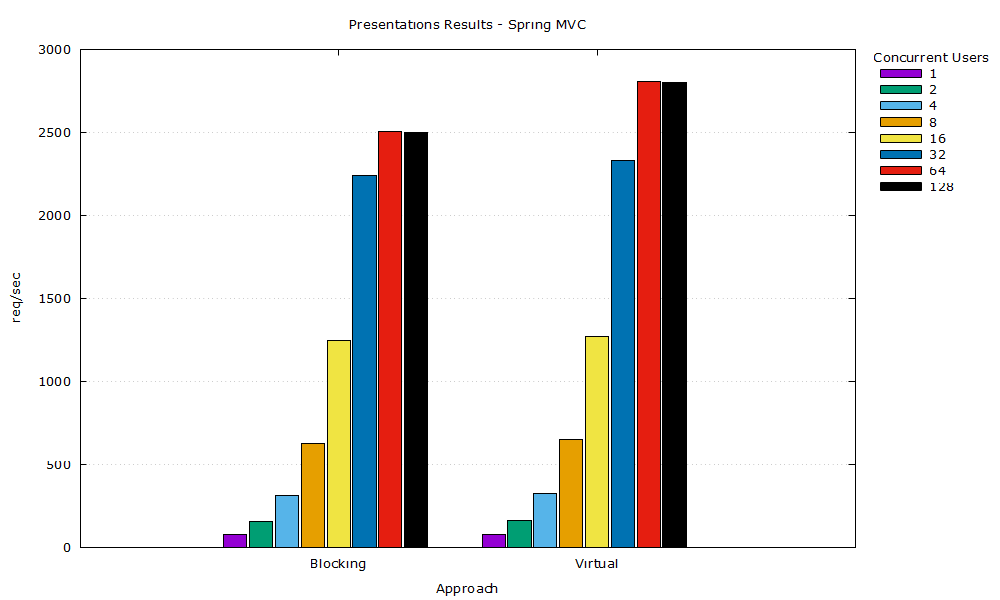
\includegraphics[width=0.8\textwidth]{./Graphs/presentations-springmvc-jmeter.png}
     \caption{Throughput (requests per second) scalability results for Spring MVC with \texttt{Presentations} class}\label{fig:presentations-springmvc-jmeter}
\end{figure}

% The results for the Spring MVC implementation, shown in
% Figure~\ref{fig:presentations-springmvc-jmeter}, compare two approaches:
% \textit{Blocking}, which uses platform threads with \texttt{StreamingResponseBody},
% and \textit{Virtual}, which uses Virtual Threads. Both approaches scale
% effectively up to 128 concurrent users, with the Virtual Thread approach
% achieving a slightly higher throughput of 9,000 requests per second. However,
% these values are slightly lower than those observed in the Spring WebFlux
% implementation.
The results for the Spring MVC implementation, shown in
Figure~\ref{fig:presentations-springmvc-jmeter}, compare two synchronous
approaches: \textit{Blocking}, which uses platform threads with
\texttt{StreamingResponseBody}, and \textit{Virtual}, which uses Virtual
Threads. Since Spring MVC follows a thread-per-request architecture, the
asynchronous approaches—\textbf{Reactive} and \textbf{Suspendable}—described in
Section~\ref{sec:bench} are not applicable. Both the \textit{Blocking} and
\textit{Virtual} strategies scale effectively up to 32 concurrent users, with
the Virtual Threads approach achieving a slightly higher maximum throughput of
2,797 requests per second, compared to 2,498 requests per second for the
blocking approach. These results indicate that while Spring MVC can handle a
moderate level of concurrency, it does not reach the scalability of the
reactive or suspendable approaches available in Spring WebFlux. Furthermore,
Spring MVC does not enable Progressive Server-Side Rendering (PSSR) for the
tested templates, as previously discussed in Section~\ref{sec:bench}.

\begin{figure}[h]
     \centering
     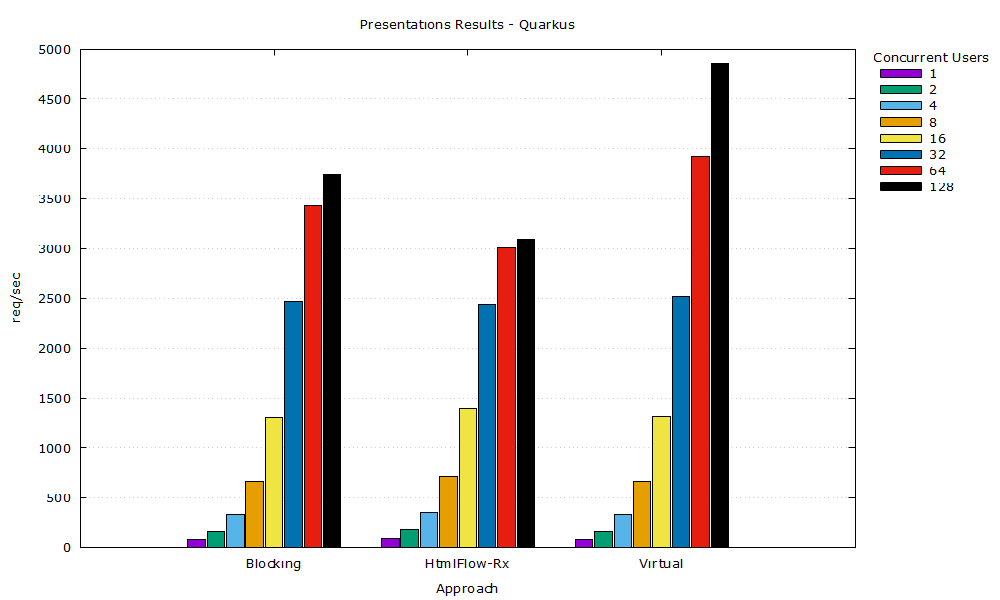
\includegraphics[width=0.8\textwidth]{./Graphs/presentations-quarkus-jmeter.png}
     \caption{Throughput (requests per second) scalability results for Quarkus with \texttt{Presentations} class}\label{fig:presentations-quarkus-jmeter}
\end{figure}

The results for the Quarkus implementation, shown in
Figure~\ref{fig:presentations-quarkus-jmeter}, indicate that Quarkus handles
synchronous approaches more efficiently than Spring WebFlux. The blocking
engines scale up to 64 concurrent users, achieving up to 3,744 requests per
second. When using Virtual Threads, the throughput increases even further,
reaching 4,856 requests per second, allowing scalability up to 128 users. This
demonstrates that Quarkus's implementation of Virtual Threads is effective for
enabling PSSR\@, and comparable to the \textit{Suspendable} and
\textit{Reactive} approaches used in Spring WebFlux in terms of scalability and
throughput.

Additionally, \textit{HtmlFlow-Rx}, a reactive implementation of the HtmlFlow
template engine (equivalent to the approach shown in
Listing~\ref{lst:presentation-observable}) that utilizes Quarkus's reactive
programming model, achieved a lower throughput than the the \textit{Blocking}
and \textit{Virtual} approaches—3,088 requests per second. This demonstrates
that Quarkus's reactive programming model is effective for enabling PSSR\@,
although it does not achieve the same level of performance or scalability as
the same approach in Spring WebFlux, stagnating after 32 concurrent users.

\subsection{Scalability results for the \texttt{Stocks} class} \label{sec:stocks-results}

\begin{figure}[h]
     \centering
     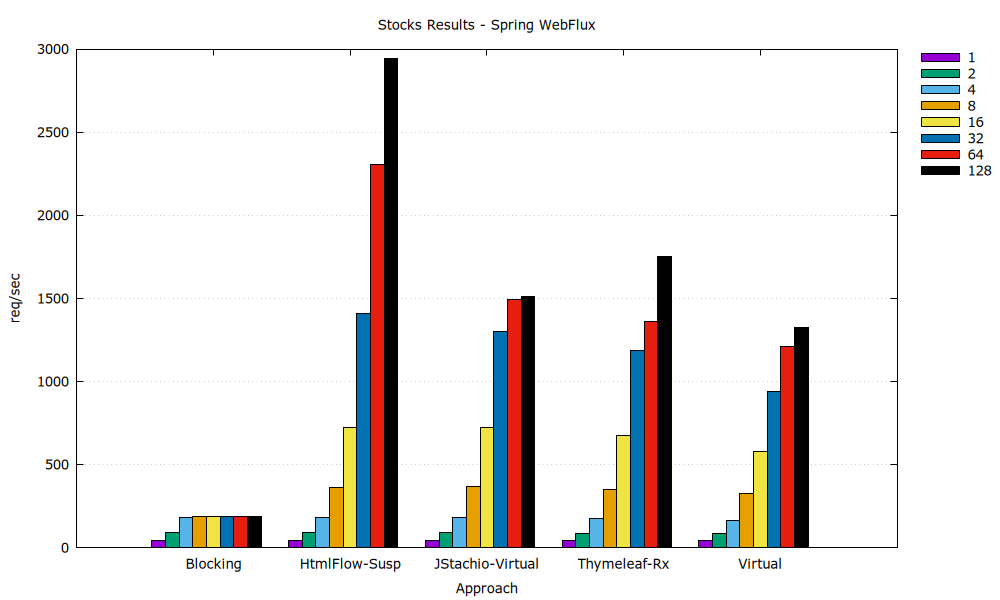
\includegraphics[width=0.8\textwidth]{./Graphs/stocks-webflux-jmeter.png}
     \caption{Throughput (requests per second) scalability results for Spring Webflux with \texttt{Stocks} class}\label{fig:stocks-webflux-jmeter}
\end{figure}

The results in Figure~\ref{fig:stocks-webflux-jmeter} use the same template
engines and approaches as the previous benchmark, but with a more complex data
model: the Stock class, which includes 20 instances and approximately two times
as many data bindings. With this data model, the scalability of the engines
remains largely unchanged; however, throughput is reduced across all engines.
Compared to the Presentation benchmark, Jstachio using virtual threads
experienced a more pronounced decrease in performance relative to the
\textit{Reactive} and \textit{Suspending} approaches, with Jstachio using
Virtual Threads now achieving 1,509 requests per second, compared to 1,750
requests per second achieved by the Thymeleaf implementation using the reactive
View Resolver driver.

It is again important to note that the differences in scalability and
throughput between the \textit{HtmlFlow-Susp}, \textit{Jstachio-Virtual}, and
\textit{Thymeleaf-Rx} approaches may be influenced by the specific template
engines used, rather than the approach itself. When comparing the
\textit{Reactive}, \textit{Suspendable}, and \textit{Virtual} approaches
specifically with HtmlFlow, we found that all three achieve similar
performance: HtmlFlow using a blocking approach with Virtual Threads reaches
3,090 requests per second, while HtmlFlow using a reactive approach achieves
3,026 requests per second. This indicates that the more pronounced decrease in
performance for Jstachio using Virtual Threads is likely due to the specific
implementation of the template engine, rather than the use of Virtual Threads
itself.

The overall throughput reduction across all engines is expected, as the Stock
class contains more data properties than the \texttt{Presentation} class,
adding overhead related to the data binding process of each template engine.

\begin{figure}[h]
     \centering
     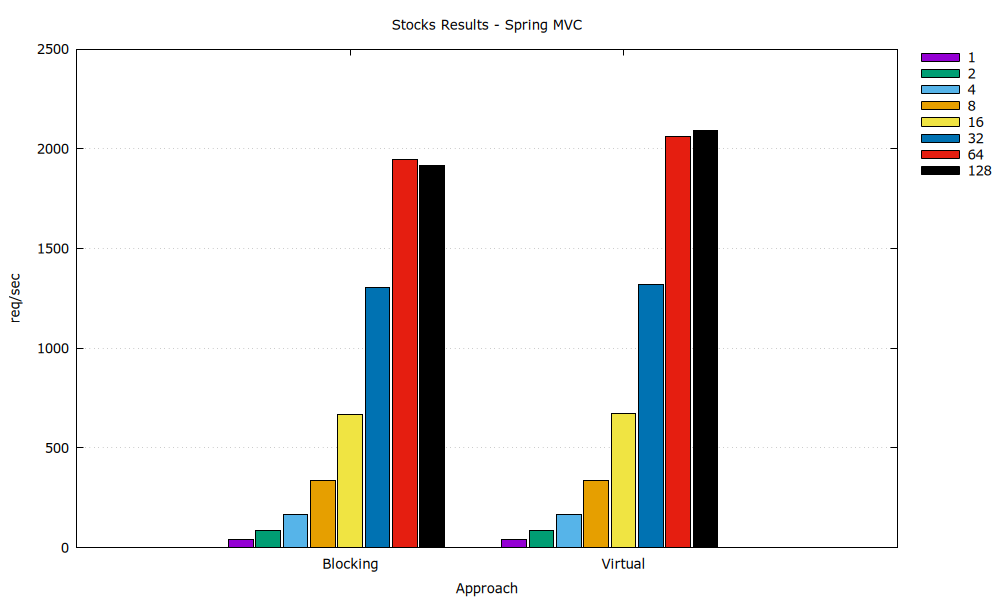
\includegraphics[width=0.8\textwidth]{./Graphs/stocks-springmvc-jmeter.png}
     \caption{Throughput (requests per second) scalability results for Spring MVC with \texttt{Stocks} class}\label{fig:stocks-springmvc-jmeter}
\end{figure}

The results shown in Figure~\ref{fig:stocks-springmvc-jmeter} indicate that the
Spring MVC implementation using the blocking approach with
\texttt{StreamingResponseBody} achieves a throughput of up to 1,916 requests
per second, with no significant improvement observed when using Virtual
Threads. Both approaches scale effectively up to 64 concurrent users. Although
these approaches achieve higher throughput in Spring MVC than in Spring
WebFlux, their overall performance remains lower than that of the reactive and
suspendable approaches.

\begin{figure}[h]
     \centering
     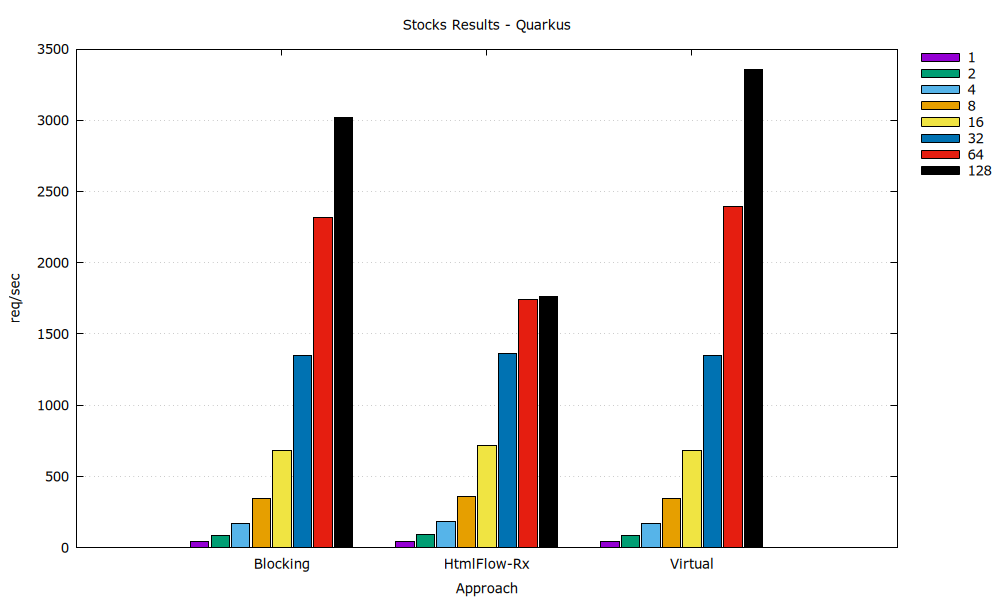
\includegraphics[width=0.8\textwidth]{./Graphs/stocks-quarkus-jmeter.png}
     \caption{Throughput (requests per second) scalability results for Quarkus with \texttt{Stocks} class}\label{fig:stocks-quarkus-jmeter}
\end{figure}

The results depicted in Figure~\ref{fig:stocks-quarkus-jmeter} show that the
Quarkus synchronous approaches scale effectively up to 128 concurrent users,
achieving performance comparable to the Spring WebFlux implementation. The
blocking approach reaches a throughput of 3,019 requests per second, while the
Virtual Threads approach achieves a throughput of 3,357 requests per second. In
addition to the synchronous engines, the \textit{HtmlFlow-Rx} approach also
achieves a throughput of 1760 requests per second, indicating that this
approach achieves lower performance in Quarkus than in Spring WebFlux, where it
reached 3,026 requests per second, as previously mentioned.

The results of the benchmarks show that non-blocking engines—whether using
reactive programming, Kotlin coroutines, or Java Virtual Threads—are able to
scale effectively, supporting between 32 and 128 concurrent users depending on
the approach and framework. Out of all the tested frameworks, Spring Webflux
showed itself the most effective at enabling PSSR, mostly due to its native
support for publish-subscribe interfaces, allowing for content to be streamed
as data becomes available, instead of when the response buffer is flushed.
Quarkus also enabled PSSR effectively, but it required additional configuration
of the \texttt{OutputBuffer} size to achieve the same results as Spring
Webflux. The Spring MVC implementation, on the other hand, did not enable PSSR
for the tested templates.

However, it is important to acknowledge the limitations of our chosen data
models for generalizability. The tested templates used relatively simple data
structures with limited nesting and straightforward property bindings.
Real-world applications often involve deeply nested data structures, complex
conditional logic, and iterative rendering over thousands of items. Under such
conditions, we anticipate significantly different performance characteristics:
increased memory consumption due to object traversal overhead, higher CPU
utilization for complex evaluations, and altered scalability patterns where
non-blocking approaches may become more advantageous. The performance
degradation observed with our Stock class benchmark—which merely doubled the
number of properties—suggests that higher template complexity would result in
substantially higher performance degradation. Future work should investigate
these scenarios with more realistic data models to better understand
performance boundaries and optimization strategies for complex PSSR
implementations.

\subsection{Memory Consumption and Resource Utilization Analysis}
\label{sec:memory-analysis}

This section evaluates the memory and CPU resource usage characteristics of
structured concurrency approaches, specifically comparing Virtual Threads and
suspendable coroutines.

Resource utilization data was collected using VisualVM during 30-second
benchmark runs, capturing detailed CPU and memory usage patterns under
sustained load conditions. Each profiling session monitored system performance
during the 1 to 128 concurrent user load test, providing comprehensive insights
into runtime behavior.

\subsubsection{Virtual Threads vs Structured Concurrency}

\begin{center}
     \begin{minipage}[t]{0.48\textwidth}
          \centering
          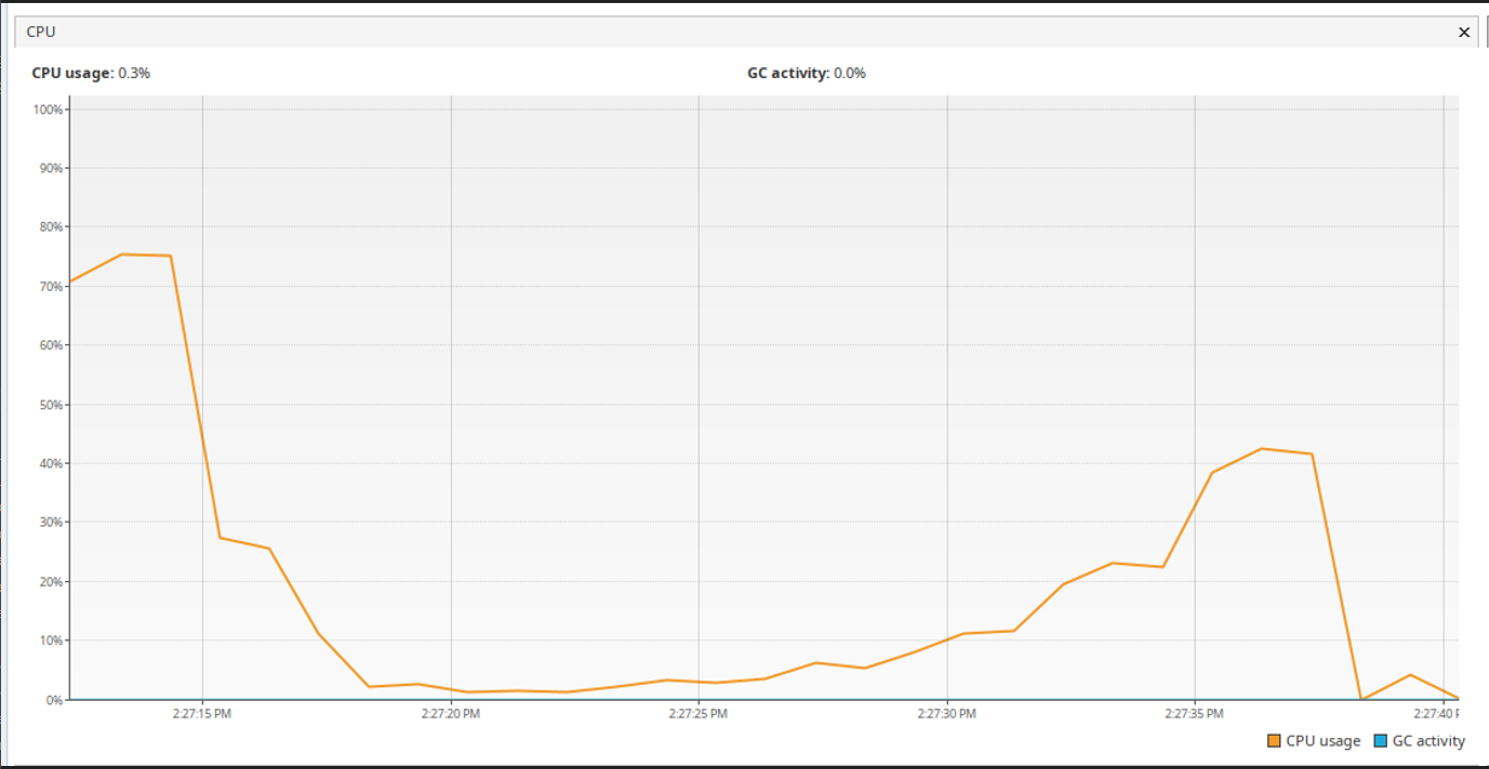
\includegraphics[width=1.0\textwidth,height=1.0\textwidth]{./Graphs/cpu-susp.png}
          \captionof{figure}{CPU utilization profiling with HtmlFlow-Susp in Spring WebFlux during 30-second load test}
          \label{fig:cpu-susp}
     \end{minipage}
     \hfill
     \begin{minipage}[t]{0.48\textwidth}
          \centering
          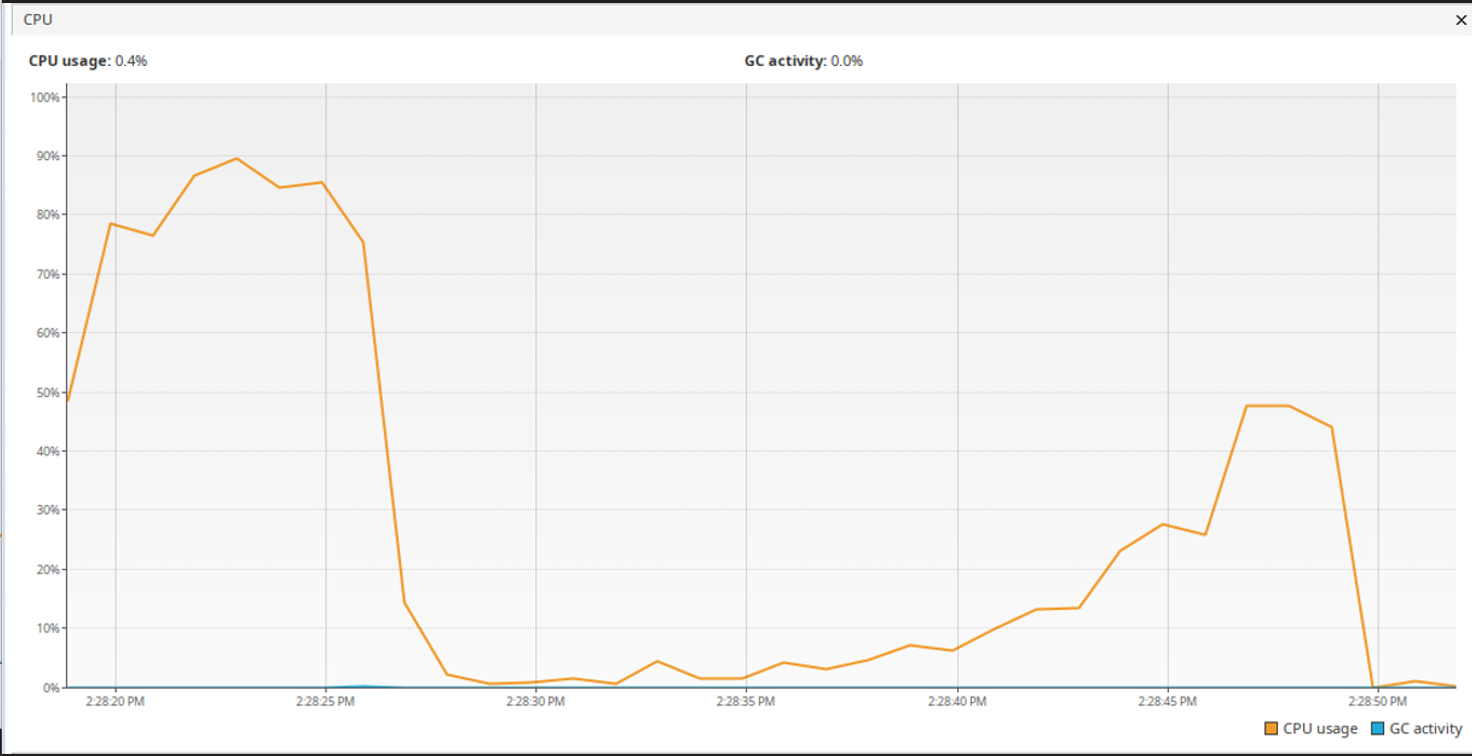
\includegraphics[width=1.0\textwidth,height=1.0\textwidth]{./Graphs/cpu-virt.png}
          \captionof{figure}{CPU utilization profiling with HtmlFlow-Virtual in Spring WebFlux during 30-second load test}
          \label{fig:cpu-virt}
     \end{minipage}
\end{center}

\begin{center}
     \begin{minipage}[t]{0.48\textwidth}
          \centering
          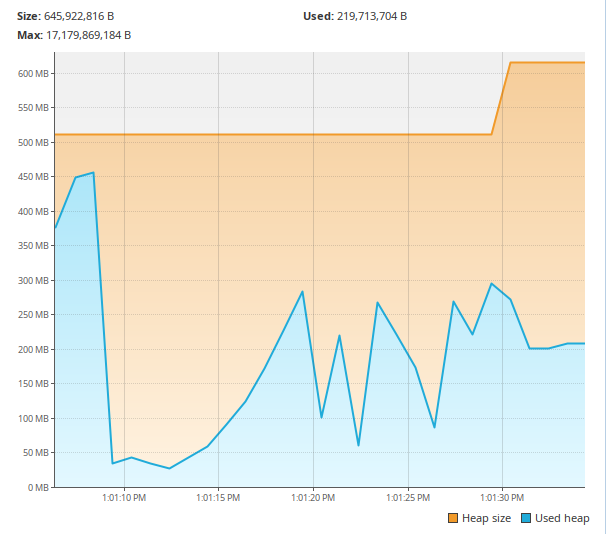
\includegraphics[width=1.0\textwidth,height=1.0\textwidth]{./Graphs/mem-susp.png}
          \captionof{figure}{Memory utilization and garbage collection behavior with HtmlFlow-Susp in Spring WebFlux during 30-second load test}
          \label{fig:gc-susp}
     \end{minipage}
     \hfill
     \begin{minipage}[t]{0.48\textwidth}
          \centering
          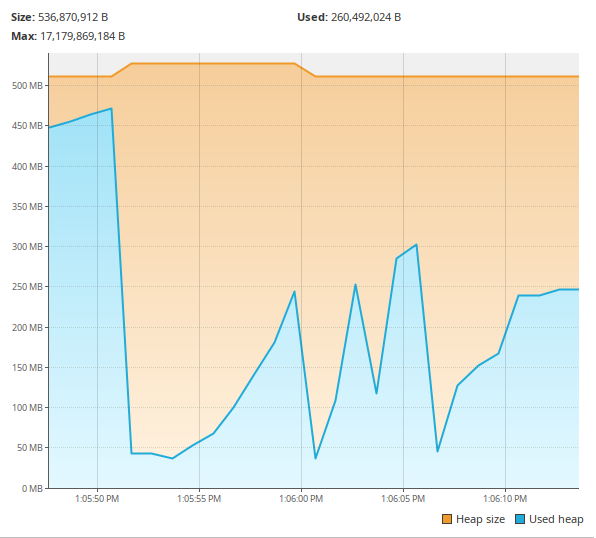
\includegraphics[width=1.0\textwidth,height=1.0\textwidth]{./Graphs/mem-virt.png}
          \captionof{figure}{Memory utilization and garbage collection behavior with HtmlFlow-Virtual in Spring WebFlux during 30-second load test}
          \label{fig:gc-virt}
     \end{minipage}
\end{center}

Figures~\ref{fig:cpu-virt} and~\ref{fig:cpu-susp} show CPU utilization profiles
for the \texttt{HtmlFlow-Virtual} and \texttt{HtmlFlow-Susp} implementations,
respectively. The subsequent gradual increase in CPU utilization reflects the
ramp-up of concurrent users during the benchmark. \texttt{HtmlFlow-Virtual}
exhibits a distinctive bell-shaped curve, rapidly climbing from near-zero to
peak CPU usage of around 50\% during the sustained load phase, maintaining
moderate utilization during the test period, and then dropping sharply back to
baseline. \texttt{HtmlFlow-Susp} displays a similar pattern but with a slightly
lower peak CPU utilization of approximately 42\%, showing marginally lower
intensive CPU usage during the sustained load phase. Both profiles demonstrate
comparable resource consumption patterns, with the virtual thread
implementation showing only slightly higher CPU demands. The GC activity
indicators in both profiles remain relatively low throughout the test duration,
confirming that garbage collection overhead does not significantly impact CPU
utilization in either approach.

Figures~\ref{fig:gc-susp} and~\ref{fig:gc-virt} show similar memory usage for
both approaches, with peaks around 300~MB during load. The initial spike to
450~MB in both graphs corresponds to the applications' bootstrapping phase.
Overall, these results indicate that under the tested conditions, Virtual
Threads and suspendable coroutines exhibit comparable memory consumption.

Virtual Threads allocate a full call stack per thread, which is unmounted and
stored on the heap when suspended (e.g., during blocking I/O). In contrast,
Kotlin coroutines compile into state machines that capture only the minimal
execution state needed to resume computation. This typically allows coroutines
to scale more efficiently in terms of memory usage, especially under high
concurrency. 

\section{Discussion}

Beronić et al.~\cite{9803765} compared different structured concurrency constructs 
in Java and Kotlin in the context of a multithreaded HTTP server. 
Their benchmark scenario differs from ours: their server awaited incoming requests 
and, upon receiving one, executed a task involving object creation, writing the 
object's information to a file, and returning the data as a response.
Consistent with our findings, they concluded that both Kotlin's coroutines and 
Java's virtual threads offer significant performance improvements over traditional 
JVM-based threads in concurrent applications.

However, our results diverge from theirs regarding memory usage. 
They reported lower heap usage for Java virtual threads (16–64~MB) compared to 
Kotlin coroutines (52–99~MB), which contrasts with our measurements. 
This discrepancy may be attributed to the different workloads: while their 
benchmark includes a single I/O read-write operation per request, our experiments 
focus exclusively on read-only I/O tasks.

The work of Navarro et al.~\cite{navarro2023considerations} focused on the
performance of Quarkus, which relies on Eclipse Vert.x~\cite{vertx}, itself
built on top of Netty~\cite{netty}. 
This represents a similar environment to the one evaluated in our experiments
with Quarkus. 
Their study also emphasized template rendering, using a blocking HTML template
engine (Qute). 
The benchmark they employed is the Fortunes
test\footnote{\url{https://www.techempower.com/benchmarks}}, which involves
rendering a simple HTML table with only two data bindings per row.

Their results show that Quarkus with Virtual Threads outperformed the
traditional thread-per-request model under increased concurrency. Moreover,
compared to the reactive model, virtual threads demonstrated competitive
performance, particularly when executing blocking operations within template
engines.
In contrast, our experiments revealed that the reactive approach underperforms 
relative to virtual threads, likely due to the significantly larger number of 
data bindings in our use cases—namely, the \texttt{Presentation} and \texttt{Stock} 
models.

The work of Šimatović et al.\cite{vsimatovic2025evaluating} presents an
evaluation of Java Virtual Threads under different garbage collectors. They
explored three types of workloads, only one of which was based on a web
application scenario. This scenario replicated large-scale web scraping by
executing 1,000 parallel tasks, each consisting of an I/O-bound operation
followed by CPU-bound string processing.

In this workload, garbage collection activity remained low across all 
collectors, indicating reduced memory pressure. These findings suggest 
that Virtual Threads improve memory allocation efficiency and reduce the 
frequency of garbage collection cycles—particularly when used with 
concurrent garbage collectors.

Our observations suggest that the choice between Virtual Threads and
suspendable coroutines should be guided by both runtime behavior and
development preferences. Virtual Threads offer the simplicity of synchronous
programming with competitive performance in moderate-load scenarios. In
contrast, suspendable coroutines, while requiring an asynchronous programming
model, may offer better efficiency in applications with higher concurrency,
deeper stacks, or more dynamic workloads.